\documentclass[pageno]{jpaper}

% Change to current semester and year, e.g.:
% \newcommand{\IWreport}{Spring 2020}
\newcommand{\IWreport}{Spring 2023}
\newcommand{\quotes}[1]{``#1''}


\widowpenalty=9999

\usepackage[normalem]{ulem}
\usepackage{algpseudocodex}
\usepackage{algorithm}
\usepackage{amsfonts}
\usepackage{amsmath}
\usepackage{siunitx}

\begin{document}

\title{A Visual Modeling Tool for Trajectory Planning for Autonomous Quadrotors}

\author{Arti Schmidt \\ Adviser: Zachary Kincaid}

\date{}
\maketitle

\thispagestyle{empty}
\doublespacing
\begin{abstract}
This project develops an algorithm for generating quadrotor trajectories for freestyle flight, motivated by the goal of allowing autonomous quadrotors to track such trajectories. The algorithm takes a greedy approach, and builds on an existing method for generating very simple trajectories. It also develops a graphical tool for users to visually model these trajectories and interface with the trajectory generator. This makes trajectory planning accessible for anybody, and makes the algorithm useful for real applications. Results are presented which demonstrate the effectiveness of the approach both qualitatively and quantitatively, and also showcase the features of the modeling tool.
\end{abstract}

\section{Motivation}

Drones are a ubiquitous type of robot today. They are extremely versatile, and can do everything from hovering to cruising at speeds well over \qty{100}{km/h}, accelerate at \qty{4}{g}, perform inverted acrobatic maneuvers, and operate in both cluttered urban environments and wide open landscapes. Their wide range of flight capabilities have led to applications in videography, inspection, search and rescue, and many others, plus the creation of activities centered around the drones themselves, like drone racing and freestyle flight, which are done for entertainment and competition. As drones have become increasingly powerful and valuable for various industries, their level of autonomy has also increased to match. Pilots can now rely on features like obstacle avoidance, object following, and autonomous flight between waypoints, and tasks requiring even higher levels of autonomy like flying in locations with poor signal and repetitive tasks like package delivery are also becoming possible.

Freestyle flight is a popular activity for drone hobbyists, in which the pilot showcases their ability or the beauty of the surroundings by recording flights from a camera onboard the drone. Freestyle flight is quite a general term that can encompass many styles of flight, including everything from rapidly dodging obstacles in an indoor environment and diving alongside buildings to long range flight along mountainsides and cruising just above bodies of water. Like many other applications of drones, freestyle flight has historically been squarely in the domain of human pilots, especially because it is in many ways an artistic endeavor that requires both high level decision making to create an interesting and entertaining flight plan, as well as low level piloting skill to make the flight look good. It is not immediately clear whether adding any amount of autonomy to this formula could be beneficial or desirable at all. While this may indeed be an activity where humans will not be surpassed by computers for the foreseeable future, there are certainly situations in which computers may be useful for this purpose. For example, consider shooting a scene for a movie which may require precisely planned movements or a high degree of repeatability to do multiple takes. Or, a pilot may be unavailable or too expensive to hire for a small project. Or, the flight may involve being between obstacles at long range, where a loss of signal and crash would be likely for a human pilot. Having the ability to do autonomous freestyle flight would be invaluable in all of these cases, and as they suggest, freestyle flight can be more than just a form of entertainment. Finally, the complex and open-ended nature of freestyle flight makes it a great way to demonstrate and test the state of the art in AI and drone technology as it becomes ever more humanlike.

The goal of this project is to develop a tool that allows users to graphically model and generate freestyle trajectories for use by autonomous quadrotors. A quadrotor is simply a drone with four rotors or propellers, which is the simplest and most common type of drone, especially for freestyle flight. Trajectories are described in more detail below, but they effectively represent a quadrotor's flight path. Trajectory generation or planning is one of the three key components of many autonomous quadrotor systems \cite{hanover}. This project does not address the other two, which are perception (estimating the quadrotor's state using sensor data), and control (tracking the planned trajectory using the state estimation), but these could be integrated in future work. The project introduces a novel approach to trajectory generation designed specifically with freestyle flight in mind, and provides an open source implementation of it. A graphical modeling tool to interface with the trajectory generator is also developed. This is an important aspect of the project because even for people with substantial knowledge of the subject, a visual interface makes the application of a trajectory generation algorithm vastly more accessible. And although autonomously flying these trajectories is a very real possibility today, planning interesting ones is still an artistic, human endeavor.

\section{Background}

A trajectory is a continuous function that gives the position of a quadrotor in $\mathbb{R}^3$ at any given time. Trajectory planning for quadrotors is a hard problem because the state space is both large and high dimensional. The quadrotor's state includes position in $\mathbb{R}^3$, velocity in $\mathbb{R}^3$, and rotation in $SO(3)$, for a total of nine dimensions \cite{mueller}. And in some applications, trajectories may be planned over distances of many kilometers, while requiring a resolution on the order of centimeters in particular locations to navigate around obstacles. Furthermore, a trajectory must be feasible, meaning that it respects the quadrotor dynamics. Specifically, the amount of linear and angular acceleration that a quadrotor can produce is limited, and additional considerations like aerodynamic drag also exist for more complicated quadrotor models. And finally, additional constraints may be imposed on a trajectory, such as position constraints to ensure that the quadrotor does not pass through obstacles, or speed constraints to ensure that the quadrotor does not exceed a maximum speed in some segment.

Many methods for planning quadrotor trajectories have been proposed in the literature. These include those taking global optimization approaches, those using sampling methods, and those leveraging polynomial representations of trajectories \cite{hanover}. Many of these methods are concerned with generating time optimal and collision free trajectories, which are useful in the context of drone racing, for example. Some methods also consider other objectives, like incorporating camera perception information to best identify obstacles \cite{zhou}. Unlike the trajectories considered in these works, freestyle trajectories do not have a clear objective function to be optimized, which is a challenge discussed in more detail later. To the author's knowledge, trajectory planning for freestyle flight has not been explicitly considered before in the literature. But as noted in the introduction, freestyle flight is a term with very broad applicability and could be used to describe many types of flight trajectories, so much of freestyle trajectory generation heavily overlaps with the existing literature.

One widely cited work on quadrotor trajectory generation by Mueller et al. \cite{mueller} proposed a method for generating \quotes{motion primitives}, which are essentially simple trajectories that can be used as building blocks for creating more complex ones. A motion primitive is constrained by the quadrotor's initial and final position, velocity, and acceleration, as well as the flight duration. The final translational variables may also be left free in any dimensions. Motion primitives are fifth degree polynomial trajectories that are chosen to minimize the squared norm of their jerk while respecting the initial and final constraints. Jerk refers to the first derivative of acceleration, and as Mueller et al. explain, this cost function is \quotes{representative of the aggressiveness of the true system inputs} \cite{mueller}. This is because the control inputs are the rotor speeds, which are directly related to the quadrotor's linear and angular acceleration, and so minimizing the jerk corresponds to minimizing the change in these accelerations, and thus also roughly minimizing the control inputs. The paper derives a closed form solution for generating these motion primitives by deferring feasibility testing to a later step (instead of incorporating these constraints into the optimization problem), and solving for each spatial dimension independently \cite{mueller}. By doing so, generating motion primitives just requires evaluating a matrix multiplication along each axis. Feasibility of the motion primitive is determined by comparing the required thrust and body rates to the user supplied minimum thrust and maximum thrust and body rates. This test is applied recursively along the motion primitive with increasingly short time intervals. With this approach, \quotes{on the order of one million motion primitives per second can be generated and tested for feasibility on a laptop computer with an unoptimized implementation} \cite{mueller}, which makes it ideal for searching over many final constraints and durations to find the motion primitive which best achieves the goal. Mueller et al. provide both a Python and C++ implementation of their method \cite{generator}. This project relies heavily on the ideas presented in their paper as well as their implementation, which will largely be treated as a black box for the rest of this paper.

In addition to trajectory generation, this project also addresses the creation of a user interface for defining trajectory constraints and visualizing the resulting trajectory. This aspect of the project was inspired by a visual modeling tool for 2D trajectories created by Mceowen et al. \cite{mceowen}. In their paper, they describe and implement an optimization based approach to trajectory generation that uses successive convexification, which has had demonstrated success in applications ranging from quadrotors to rocket landing \cite{mceowen}. As they explain, formulating a problem so that this method can be applied takes a significant amount of work and knowledge of the theory, which makes it unapproachable for a typical user that would like to be able to simply specify a trajectory. To fix this, they create a visual modeling system that gives users a graphical interface for defining constraints and providing information about the resulting trajectory. Users can define positional constraints, elliptical keep out zones, and constraints like slow zones that are active only when the quadrotor is in a certain set of states.

\section{Approach}

In this project, the constraints for a trajectory are given as $C_i = (x_i, R_i, t_i)$ for all $i \in \{1, \dots, n\}$, where $n$ is variable. Constraint $C_i$ requires that the quadrotor is at position $x_i \in \mathbb{R}^3$, $t_i \in \mathbb{R}_{\geq 0}$ seconds after arriving at $x_{i-1}$. That is, $t_i$ is the flight time between $x_{i-1}$ and $x_i$, and $t_1$ is arbitrary as the quadrotor's initial position is assumed to be $x_1$. Optionally, $R_i \in SO(3)$ can be specified, which requires that the quadrotor has rotation matrix $R_i$ at $t_i$. An unconstrained rotation is denoted as $\emptyset$. Note that the trajectory generation algorithm ignores rotation about the quadrotor's yaw axis, which is discussed later. This choice of constraints should allow for the specification of a diverse range of trajectory styles, such as the trajectories found in freestyle flight. For simplicity, constraints describing keep out regions (to avoid obstacles, for example) are not supported. Instead, users can set position constraints as necessary until the generated trajectory does not intersect any of these regions. The sequence of position constraints determines the basic structure or route that the trajectory will take, which could be on the scale of meters or kilometers. Duration constraints affect the quadrotor's speed. Rotation constraints allow for controlling the direction of the quadrotor's camera and specifying acrobatic maneuvers like inversions. A trajectory for flying along a mountain ridge may only require a simple sequence of position constraints with arrival times set to achieve the desired speed. On the other hand, a trajectory for flying between buildings and other urban obstacles while performing acrobatics could make use of many position constraints to ensure that the generated trajectory closely follows a desired path, as well as rotation constraints to, for example, point downwards while diving alongside a building, keep a sculpture in view while flying around it, or be upside down when at the apex of a loop.

To generate trajectories that respect these constraints, an algorithm is developed which builds on the motion primitive library from Mueller et al. It works by reducing the generation of the full trajectory to generating a sequence of motion primitives with appropriate initial and final constraints using a greedy heuristic. This approach is chosen from among the many options described in the literature because motion primitives are simple and understandable, and the paper provides an easy to use Python implementation for generating them. Additionally, they can be made to work with the constraint model described above without modification to the underlying approach, and their optimization objective of minimal jerk is a good choice for freestyle trajectories. As mentioned previously, trajectories for freestyle flight do not need to be optimal with respect to time or any other easily apparent metric, they need only respect the given constraints. However, to the extent possible, freestyle trajectories should appear relatively smooth and natural, which makes them more enjoyable and engaging to watch. This is a challenging objective to formalize, but one possibility is to minimize some derivative of the quadrotor's position with respect to time. Because jerk roughly corresponds to the aggressiveness of the inputs to the quadrotor \cite{mueller}, it is a sensible choice for producing trajectories that look smooth. Unfortunately, the motion primitive library does lack one important feature, which is the generation of yaw angle trajectories \cite{mueller}. The quadrotor yaw angle can be considered independently of the other inputs since it is rotation about the thrust axis, and thus it is a sensible omission from the library. But, a yaw trajectory is essential for freestyle flight in particular, because this controls where the camera points, and so it is necessary for visually appealing camera footage from onboard the drone. While generating yaw trajectories could likely be a straightforward addition for this project, this was not done due to time constraints, and so the quadrotor's yaw angle is always fixed at zero.

The following notation is used regarding motion primitives for the rest of this paper. \\ $g(p_0, v_0, a_0, p_1, v_1, a_1, t)$ is the motion primitive generation function, which takes parameters, in order, for the quadrotor initial position, velocity, and acceleration; final position, velocity, and acceleration; and the motion primitive duration. It returns a trajectory object $\tau$ using Mueller et al.'s algorithm, or the value $\emptyset$ if this is infeasible. To test for feasibility, the quadrotor's minimum acceleration $f_{\min}$ (in \unit{m/s^2}), maximum acceleration $f_{\max}$ (in \unit{m/s^2}), and maximum angular rate $\omega_{\max}$ (in \unit{rad/s}) are taken as input. $x_{\tau}(t)$, $\dot x_{\tau}(t)$, $\ddot x_{\tau}(t)$, and $R_{\tau}(t)$ are functions which query for the quadrotor position, velocity, acceleration, and rotation, respectively, at a given time $t$ along trajectory $\tau$. $c(\tau)$ gives the cost of $\tau$ as defined by Mueller et al.

\begin{algorithm}
\caption{Naive}\label{alg:naive}
\begin{algorithmic}[1]
\State $x_{\tau_1}(t_1) \gets x_1$
\State $\dot x_{\tau_1}(t_1) \gets (0, 0, 0)$
\State $\ddot x_{\tau_1}(t_1) \gets (0, 0, 0)$
\State feasible $\gets$ true
\For{$i \gets 2, \dots, n$}
  \State $p_0 \gets x_{\tau_{i-1}}(t_{i-1})$
  \State $v_0 \gets \dot x_{\tau_{i-1}}(t_{i-1})$
  \State $a_0 \gets \ddot x_{\tau_{i-1}}(t_{i-1})$
  \State $p_1 \gets x_i$
  \State $v_1 \gets \text{free}$
  \State $a_1 \gets \text{free}$
  \State $t \gets t_i$
  \State $\tau_i \gets g(p_0, v_0, a_0, p_1, v_1, a_1, t)$
  \If{$\tau_i = \emptyset$}
    \State feasible $\gets$ false
  \EndIf
\EndFor
\end{algorithmic}
\end{algorithm}

Algorithm \ref{alg:naive} shows pseudocode for a naive approach to trajectory generation which is a precursor to the greedy approach discussed later. Note that this algorithm ignores all rotation constraints. The algorithm generates trajectory segments (motion primitives) $\tau_i$ for every $i \in \{2, \dots, n\}$. Segment $\tau_i$ is the trajectory between constraints $C_{i-1}$ and $C_i$. Lines 1 to 3 set initial conditions so that the first trajectory segment has a well defined initial position, velocity, and acceleration. The algorithm proceeds by computing $\tau_i$ from $\tau_{i-1}$. For the trajectory to be a continuous function, the initial position, velocity, and acceleration of segment $\tau_i$ must be equal to the final position, velocity, and acceleration of segment $\tau_{i-1}$. The final position of $\tau_i$ must be the user supplied position constraint corresponding to the end of the segment, which is $x_i$. The final velocity and acceleration of $\tau_i$ are left unconstrained, which is the defining feature of this naive approach. The duration of $\tau_i$ must be the user supplied duration constraint, which is $t_i$. Finally, the trajectory segment $\tau_i$ is generated with the appropriate arguments on line 13. Lines 14 and 15 ensure that if any segment is infeasible, then the whole trajectory will be marked as infeasible. The algorithm produces individual trajectory segments $\tau_i$, but the desired result is one trajectory passing through all constraints, $\tau$. To achieve this, the function which queries the position of the quadrotor on $\tau$, $x_{\tau}$, is defined by effectively concatenating the corresponding functions for each segment, $x_{\tau_i}$. The other query functions for a trajectory, like velocity, are defined similarly. Let $T_i = \sum_{j=2}^i t_j$ be the cumulative time elapsed at the end of trajectory segment $\tau_i$. Then,

\begin{equation*}
  x_{\tau}(t) = \begin{cases}
    x_{\tau_2}(t) & \text{if } t \in [T_1, T_2) \\
    x_{\tau_3}(t) & \text{if } t \in [T_2, T_3) \\
    \dots \\
    x_{\tau_n}(t) & \text{if } t \in [T_{n-1}, T_n] \\
  \end{cases}
\end{equation*}

The naive algorithm produces a trajectory by generating the optimal trajectory segment between position constraints at each step. That is, only the final position of each trajectory segment is fixed; the final velocity and acceleration are free and so they are chosen to minimize the cost of the trajectory segment. This may produce reasonable trajectories for some choices of constraints, but for many it does not since each segment is optimized completely independently of the following segments. For example, consider Figure \ref{fig:naive}. The first trajectory segment simply accelerates in a straight line from the first to the second position constraint. The second trajectory segment must then compensate for the quadrotor's high velocity away from the third position constraint, but this only exaggerates the problem for the third trajectory segment. The greedy algorithm introduced below solves issues with the naive algorithm like this one, and also produces trajectories that respect rotation constraints.

\begin{figure}
  \includegraphics[width=\linewidth]{data/naive.png}
  \caption{A trajectory generated using the naive algorithm. The red quadrotors are constraints, and the white curve is the trajectory. The first constraint is the one nearest to the bottom of the image.}
  \label{fig:naive}
\end{figure}

\begin{algorithm}
  \caption{Greedy}\label{alg:greedy}
  \begin{algorithmic}[1]
  \State $x_{\tau_1}(t_1) \gets x_1$
  \State $\dot x_{\tau_1}(t_1) \gets (0, 0, 0)$
  \State $\ddot x_{\tau_1}(t_1) \gets (0, 0, 0)$
  \State $x_{n+1} \gets x_n$
  \State $t_{n+1} \gets t_n$
  \State feasible $\gets$ true
  \For{$i \gets 2, \dots, n$}
    \State $\text{best\_cost} \gets \infty$
    \State $\tau_i \gets \emptyset$
    \ForAll{$(\theta, s, f) \in A \times S \times F$}

      \State $p_0 \gets x_{\tau_{i-1}}(t_{i-1})$
      \State $v_0 \gets \dot x_{\tau_{i-1}}(t_{i-1})$
      \State $a_0 \gets \ddot x_{\tau_{i-1}}(t_{i-1})$
      \State $p_1 \gets x_i$
      \State $v_1 \gets s \cdot d(x_{i-1}, x_i, x_{i+1}, \theta)$
      \If{$R_i \neq \emptyset$}
        \State $a_1 \gets f \cdot (0, 0, 1) R_i^\top + (0, 0, -9.81)$
      \Else
        \State $a_1 \gets \text{free}$
      \EndIf
      \State $t \gets t_i$
      \State $\sigma \gets g(p_0, v_0, a_0, p_1, v_1, a_1, t)$
      \State

      \State $p_0' \gets x_{\sigma}(t_i)$
      \State $v_0' \gets \dot x_{\sigma}(t_i)$
      \State $a_0' \gets \ddot x_{\sigma}(t_i)$
      \State $p_1' \gets x_{i+1}$
      \State $v_1' \gets \text{free}$
      \State $a_1' \gets \text{free}$
      \State $t' \gets t_{i+1}$
      \State $\sigma' \gets g(p_0', v_0', a_0', p_1', v_1', a_1', t')$
      \State

      \State $\text{cost} \gets c(\sigma) + c(\sigma')$
      \If{$\sigma \neq \emptyset$ and $\sigma' \neq \emptyset$ and cost $<$ best\_cost}
        \State best\_cost $\gets$ cost
        \State $\tau_i \gets \sigma$
      \EndIf
    \EndFor
    \If{$\tau_i = \emptyset$}
      \State feasible $\gets$ false
    \EndIf
  \EndFor
  \end{algorithmic}
  \end{algorithm}

Algorithm \ref{alg:greedy} shows pseudocode for the greedy approach. Unlike Algorithm \ref{alg:naive}, the final velocity and acceleration vectors are not left free. Instead, the algorithm searches over many candidate vectors by enumerating all combinations of velocity angles $\theta$, velocity magnitudes $s$, and acceleration magnitudes $f$. However, the final acceleration is only fixed if a rotation constraint is enforced. The reasoning for parameterizing candidates this way is given below. These values are used to compute the trajectory segment $\sigma$. Then, a second trajectory segment $\sigma'$ is generated, the \quotes{induced} trajectory, which starts from the final position, velocity, and acceleration of $\sigma$. It ends at the next position constraint $x_{i+1}$, and has a free final velocity and acceleration. The cost associated with a choice of $(\theta, s, f)$ is the sum of the costs for $\sigma$ and $\sigma'$, computed on line 32. If $\sigma$ and $\sigma'$ are both feasible and the cost is better than the best seen so far, $\tau_i$ is updated to be $\sigma$.

Intuitively, this algorithm considers the cost of the induced trajectory segment $\sigma'$ to approximate how a particular choice of the current trajectory segment $\sigma$ will affect the cost of the remainder of the trajectory. It greedily chooses the segment that gives the best sum of costs, which is sensible because the cost is an integral over the trajectory, and therefore additive. As shown in the results, even looking ahead by one segment in this manner significantly improves the generated trajectories. At each $i$, the candidates for $v_1$ are sampled from a disk with radius $v_{\max}$ in the plane defined by $x_{i-1}$, $x_i$, and $x_{i+1}$. This is done to reduce the search space, as in most cases one would expect it to be unnecessary for the quadrotor to leave this plane by a large amount in a trajectory with minimal jerk. $v_1$ is computed on line 15, where $d(x_{i-1}, x_i, x_{i+1}, \theta)$ is a function giving the normalized vector $x_i - x_{i-1}$ rotated by angle $\theta$ in the plane defined by $x_{i-1}$, $x_i$, and $x_{i+1}$. $A$ is the set of angles to search over, and $S$ is the set of speeds to search over. In the implementation, these are linearly spaced values in the intervals $[0, 2\pi)$ and $[0, v_{\max}]$, respectively, where $v_{\max}$ is a parameter. If $R_i$ is enforced, then the candidates for $a_1$ have a fixed direction and variable magnitude because a quadrotor produces thrust in a direction dependent on its rotation. Its total acceleration is its thrust vector plus the effect of gravity, which is computed on line 17. $F$ is the set of thrusts to search over, which in the implementation are linearly spaced values in the interval $[f_{\min}, f_{\max}]$.

\section{Implementation}

The project is implemented as two separate components, the trajectory engine \footnote{https://github.com/arcturus3/trajectory-engine} and the trajectory renderer \footnote{https://github.com/arcturus3/trajectory}. The trajectory engine is responsible for generating and querying trajectories using the algorithm described in the approach section. Mueller et al. provided both a Python and C++ implementation of their motion primitive generation library, and I chose to work in Python to maximize iteration speed and understandability. Running time was not a major consideration as the trajectory generation does not need to be realtime, and so the slow execution speed of Python was not a significant downside, although this may become an issue for generating trajectories with many constraints and a large parameter search space. The motion primitive library is included in the project as a Git submodule. The \texttt{RapidTrajectory} class represents a motion primitive. It has a number of methods, including those for generation, for retrieving the cost and other properties of the motion primitive, and for querying the quadrotor's position, velocity, acceleration, and required thrust and body rates at any time along the motion primitive. The engine consists of a \texttt{Constraint} class, which simply holds position, rotation, and duration constraint information (note that the implementation uses cumulative arrival times instead of durations), and a \texttt{Trajectory} class, which contains some constant definitions, methods implementing Algorithms \ref{alg:naive} and \ref{alg:greedy} as described above, and methods to query the quadrotor's state at any time along the full trajectory by querying the appropriate trajectory segment.

\begin{figure}
  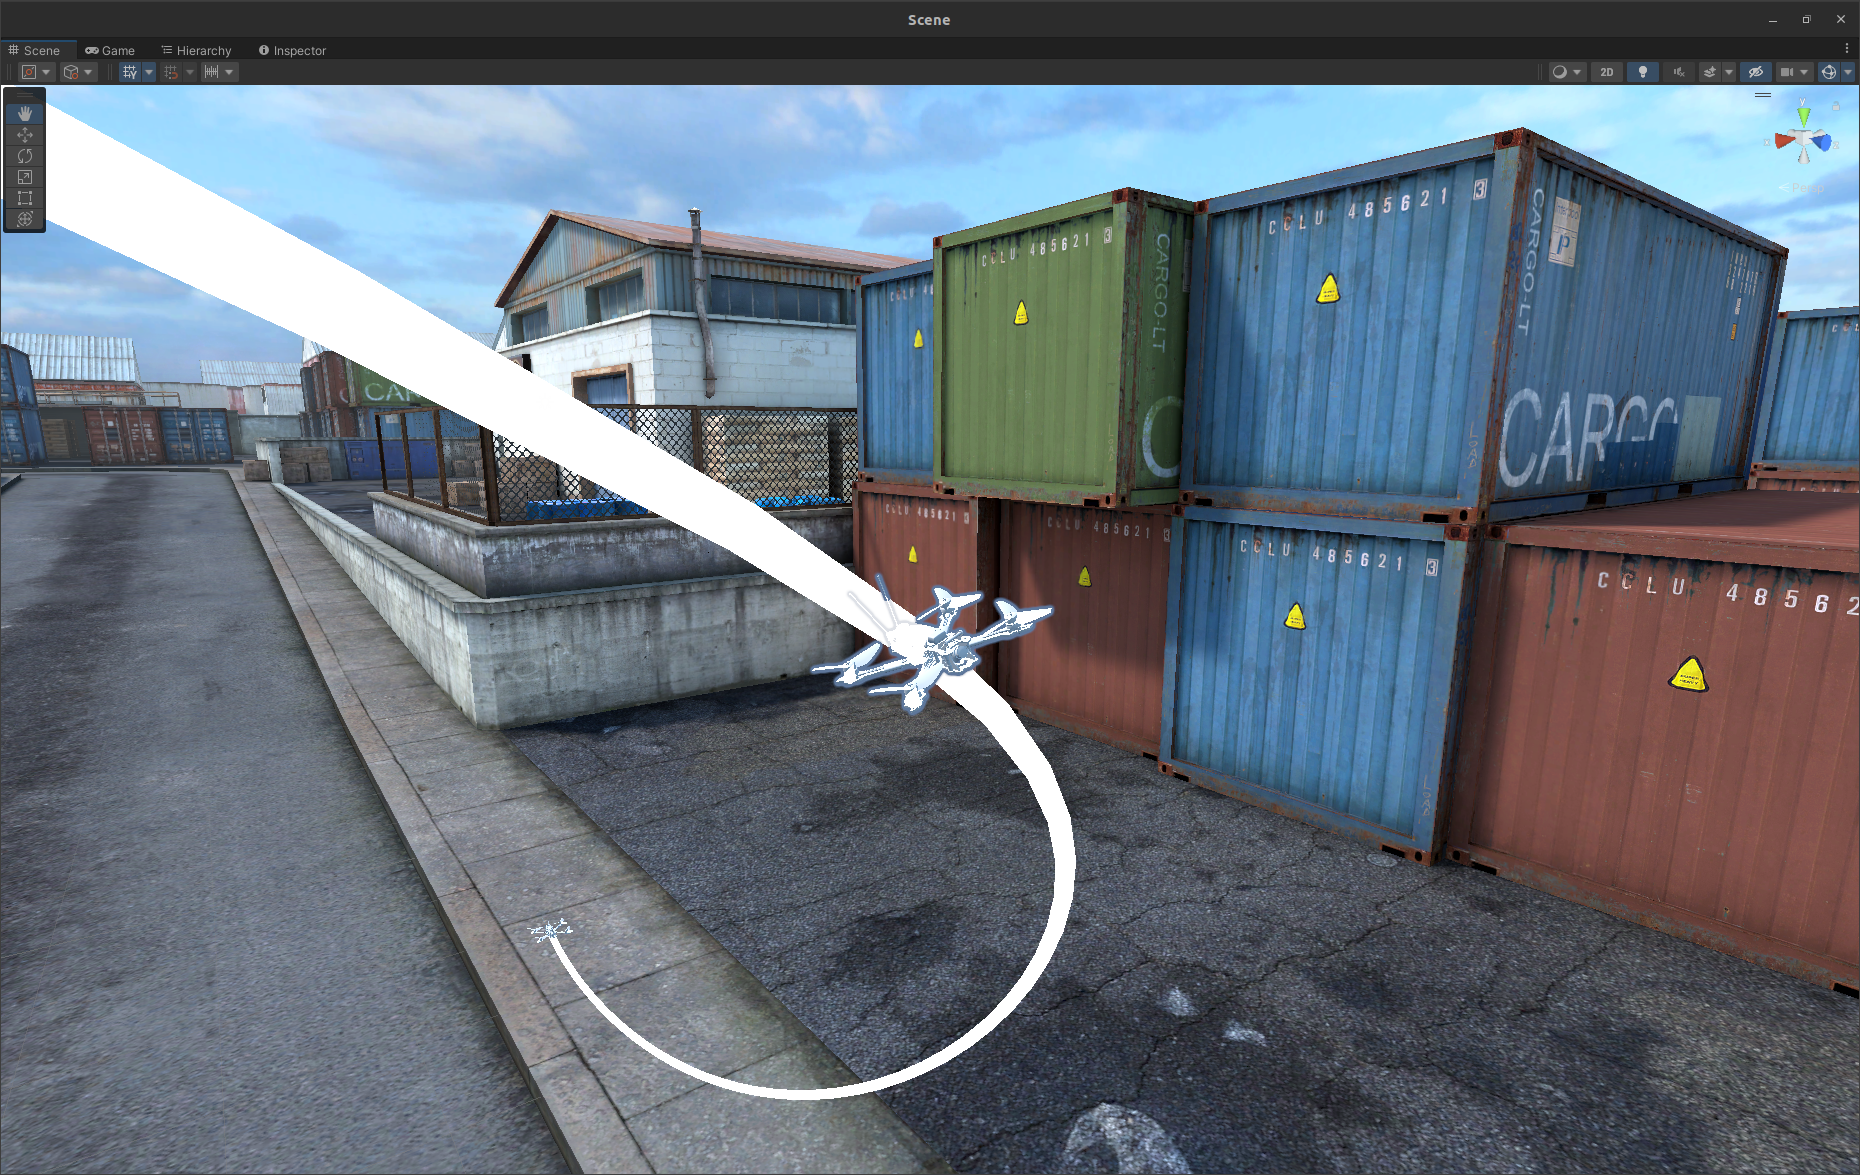
\includegraphics[width=\linewidth]{data/constraint.png}
  \caption{A \texttt{Constraint} object in the trajectory renderer. The quadrotor model has the position and rotation specified in the constraint to visualize it in 3D. This particular constraint does enforce the rotation constraint, but others may not. The white curve shows the path taken by the trajectory.}
  \label{fig:constraint}
\end{figure}

The trajectory renderer is responsible for providing a graphical interface to the user that allows them to define constraints visually, see trajectories generated from these constraints, and watch how a quadrotor would track these trajectories. The renderer is implemented using the Unity game engine \cite{unity}, which is one of the most popular platforms for 3D application development. Unity has many features that allow developers to visually edit objects in a scene in addition to controlling them at runtime via C\# scripts. To define a trajectory's constraints, users create instances of \texttt{Constraint} objects as children of a \texttt{Trajectory} object at edit time. \texttt{Constraint} objects display a quadrotor model in the scene \cite{model} as shown in Figure \ref{fig:constraint}, and Unity's \quotes{transform handles} allow the user to move and rotate the constraint in world space with their mouse. An inspector window enables the user to directly set a \texttt{Constraint}'s position $x_i$ and rotation $R_i$, as well as set its arrival time $T_i$ and indicate whether the rotation constraint should be enforced. Leveraging the Unity editor for the constraint definition task significantly reduces the number of features that need to be implemented, so this was done to simplify the project. To visualize trajectories, a script communicates with the trajectory engine to generate a trajectory from the user constraints, and the trajectory position values $x_\tau$ are then queried at a small, fixed timestep. The resulting points are rendered as a sequence of line segments using Unity's built in line renderer component. With a small enough timestep, the trajectory appears as a smooth curve in 3D space showing the path that the quadrotor will take. If the trajectory engine reports that a feasible trajectory cannot be generated from the given constraints, a warning is logged to Unity's console and the trajectory is not rendered. To see a quadrotor tracking a trajectory, the user must first define constraints and generate the trajectory. An object displaying a quadrotor model is instantiated at the start of the trajectory, and the user can press a button to start tracking. At each frame update call during tracking, a script queries the trajectory engine for $x_\tau(t)$ and $R_\tau(t)$, where $t$ is the elapsed time since tracking started. Then, the quadrotor object's position and rotation are updated with the results of the query. Tracking stops after the full duration of the trajectory has elapsed or the user presses a button to stop tracking. The user can either watch the quadrotor from an external and freely movable camera, or from a camera positioned onboard the quadrotor. In addition to the constraints, trajectory, and quadrotor, an environment is also rendered in the scene to give a sense of scale, and to present obstacles and scenery around which the user can construct the trajectory. The environment included in the project is an industrial location, which was free on the Unity asset store \cite{scene}.

The trajectory engine and trajectory renderer communicate over a ZeroMQ socket using TCP. ZeroMQ is a widely used, open source, and high speed messaging library \cite{zmq}. It is used in this project because it is a simple way to do fast interprocess communication, even though the engine and renderer were run on the same machine for all development and testing. The main requirement for the communication system was that the trajectory renderer be able to query for trajectory information in realtime, as it is tracked by the quadrotor at each frame update, which this system achieves. A request-reply pattern is used, with the engine acting as the server and the renderer acting as the client. A custom message protocol is created, which supports trajectory generation operations and trajectory query operations. Messages are serialized as JSON. The trajectory engine includes a server script to listen for and respond to incoming messages as described above. The trajectory renderer has a \texttt{Client} class to handle communication, which includes substantial code for serializing and deserializing messages, as well as converting between the coordinate system used by Unity and the coordinate system used by the motion primitive library and the trajectory engine.

\section{Results}

\begin{figure}
  \centering
  \includegraphics[width=0.75\linewidth]{data/overview.png}
  \caption{A complex trajectory generated using the greedy algorithm. White quadrotors represent constraints, although they are hard to see from this perspective, and the white curve is the trajectory. The first constraint is the one nearest to the bottom of the image.}
  \label{fig:overview}
\end{figure}

\begin{figure}
  \centering
  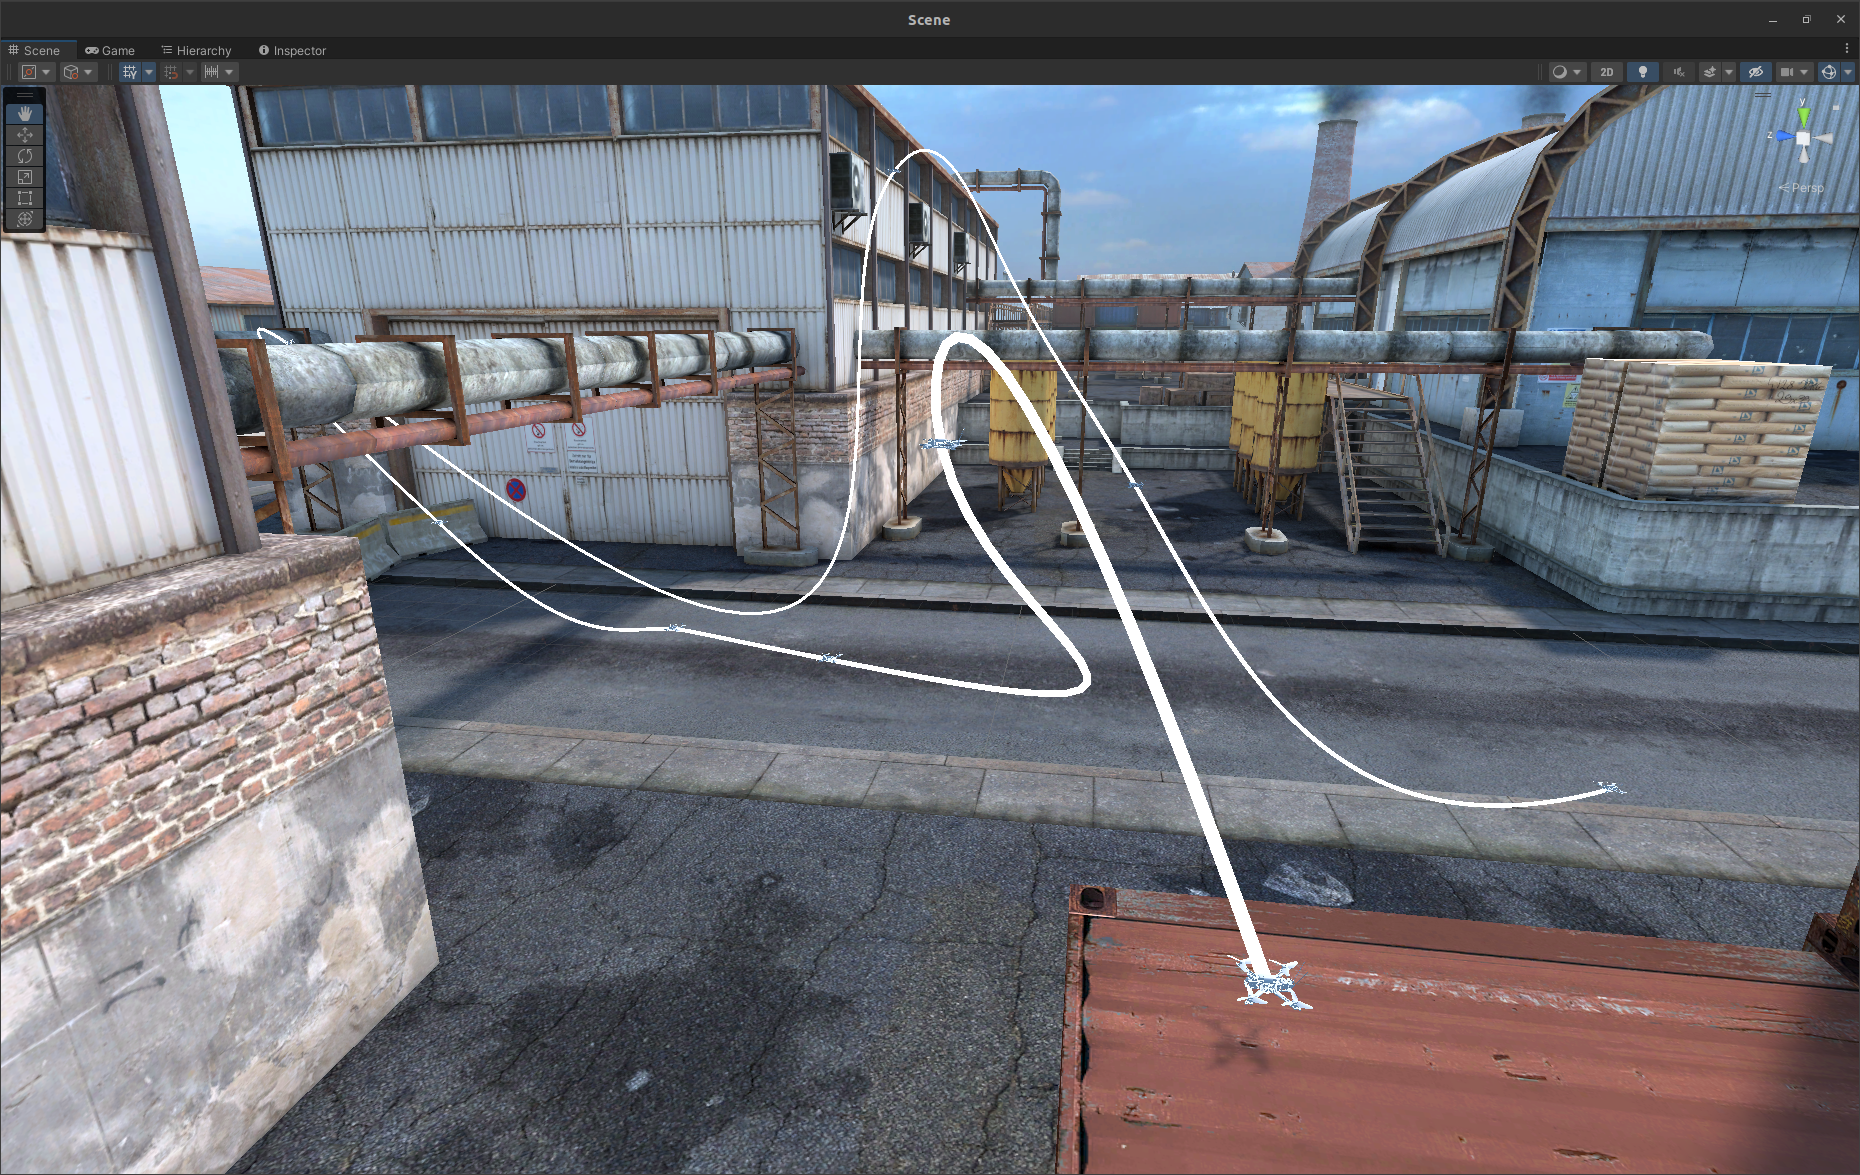
\includegraphics[width=0.75\linewidth]{data/landing.png}
  \caption{A close up view of the end of the same trajectory shown in Figure \ref{fig:overview}. This angle clearly shows the complexity of the trajectory, including its change in altitude.}
  \label{fig:landing}
\end{figure}

The approach described in Algorithm \ref{alg:greedy} is able to produce a wide variety of qualitatively interesting and visually appealing trajectories. Figure \ref{fig:overview} shows a trajectory generated from nine constraints. The total flight time is \qty{25}{s}, and the duration between constraints varies so that the quadrotor flies quickly through some sections and slowly through others. Unless noted otherwise, all trajectories were generated with parameters $|A| = 25$, $|S| = 50$, $|F| = 25$, $f_{\min} = 0$, $f_{\max} = 35$, $\omega_{\max} = 20$, and $v_{\max} = 25$. As mentioned previously, the generation algorithm does not account for obstacles in the environment, so the industrial scene just provides context and realism for the designer of the trajectory. For this trajectory, constraints were strategically placed so that it passed under the elevated pipe instead of intersecting it, for example. The trajectory is dynamic and winding, but still looks quite smooth and natural to fly, which is even more apparent when watching a quadrotor track the trajectory in a video \footnote{See video: https://drive.google.com/file/d/1GGhvepiOKyQiuS-Q-V\_gDFPm69WN65nc/view?usp=sharing}. Figure \ref{fig:landing} shows a close up view of the end of the trajectory, and emphasizes its significant change in altitude \footnote{See video: https://drive.google.com/file/d/1Aqa7HTNLoc\_kI60YJ14a9MxLAHAoN2XD/view?usp=sharing}.

\begin{figure}
  \centering
  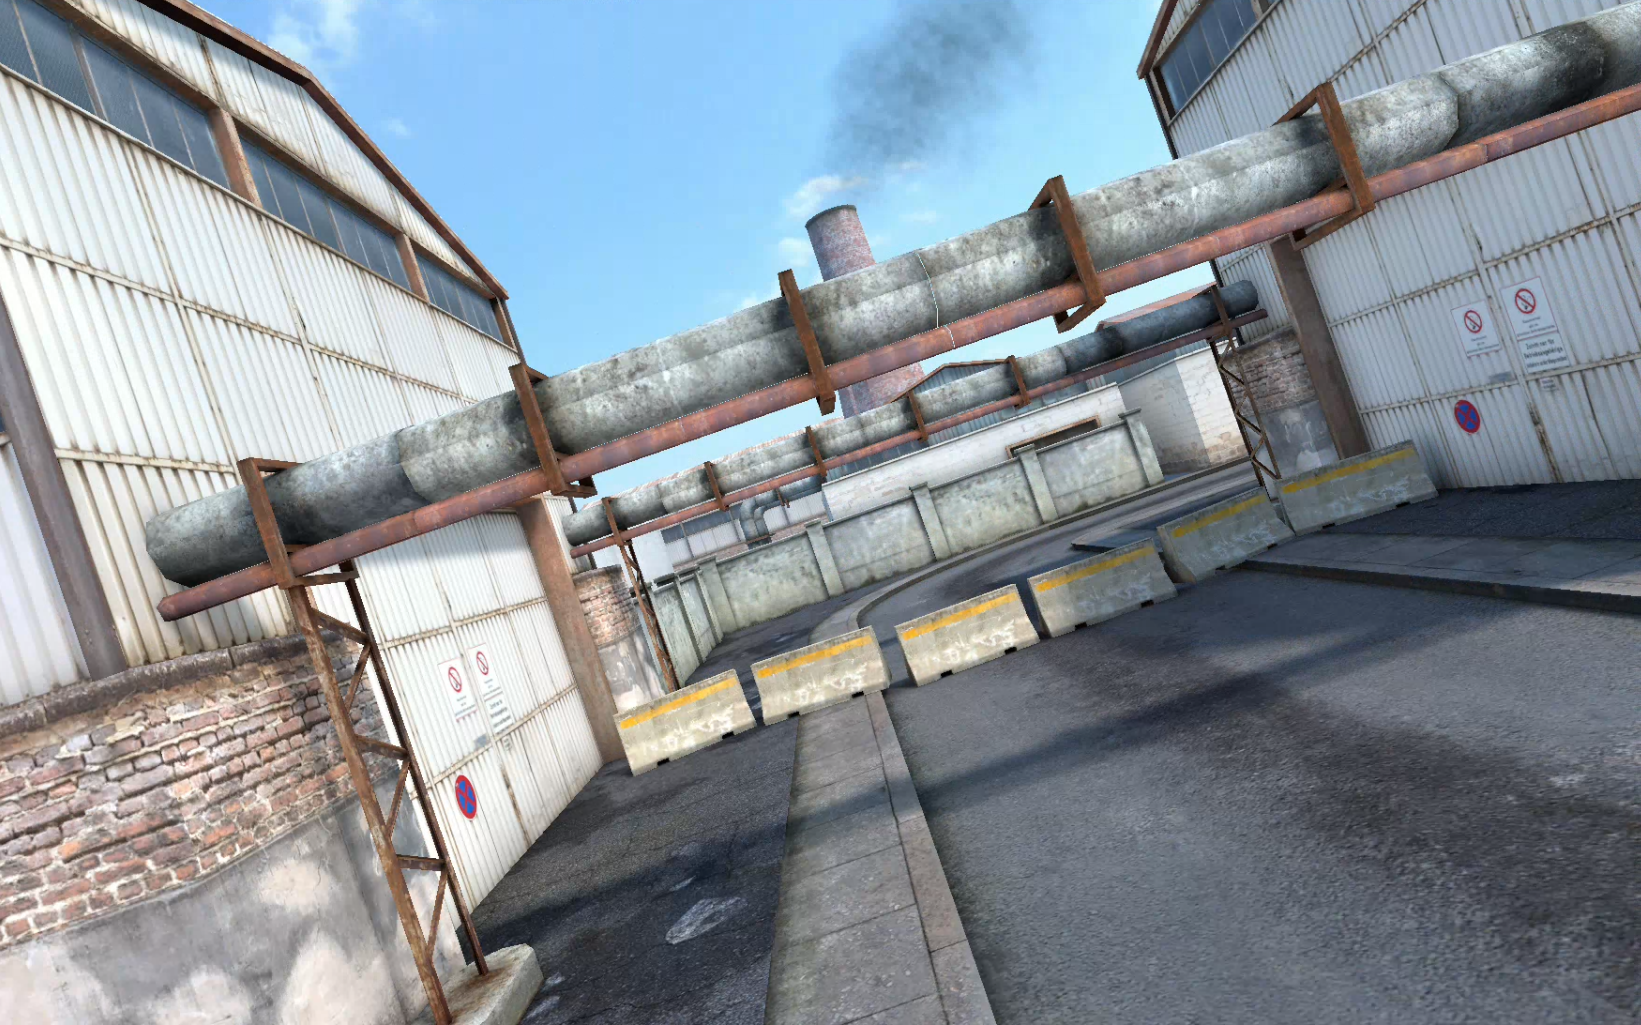
\includegraphics[width=0.75\linewidth]{data/onboard.png}
  \caption{A frame of a video taken from a camera onboard a quadrotor while tracking the trajectory shown in Figure \ref{fig:overview}. At this point in the trajectory the quadrotor is in the vicinity of a constraint which fixes its rotation. To respect this constraint, the quadrotor is noticeably rolled to the right.}
  \label{fig:onboard}
\end{figure}

\begin{figure}
  \centering
  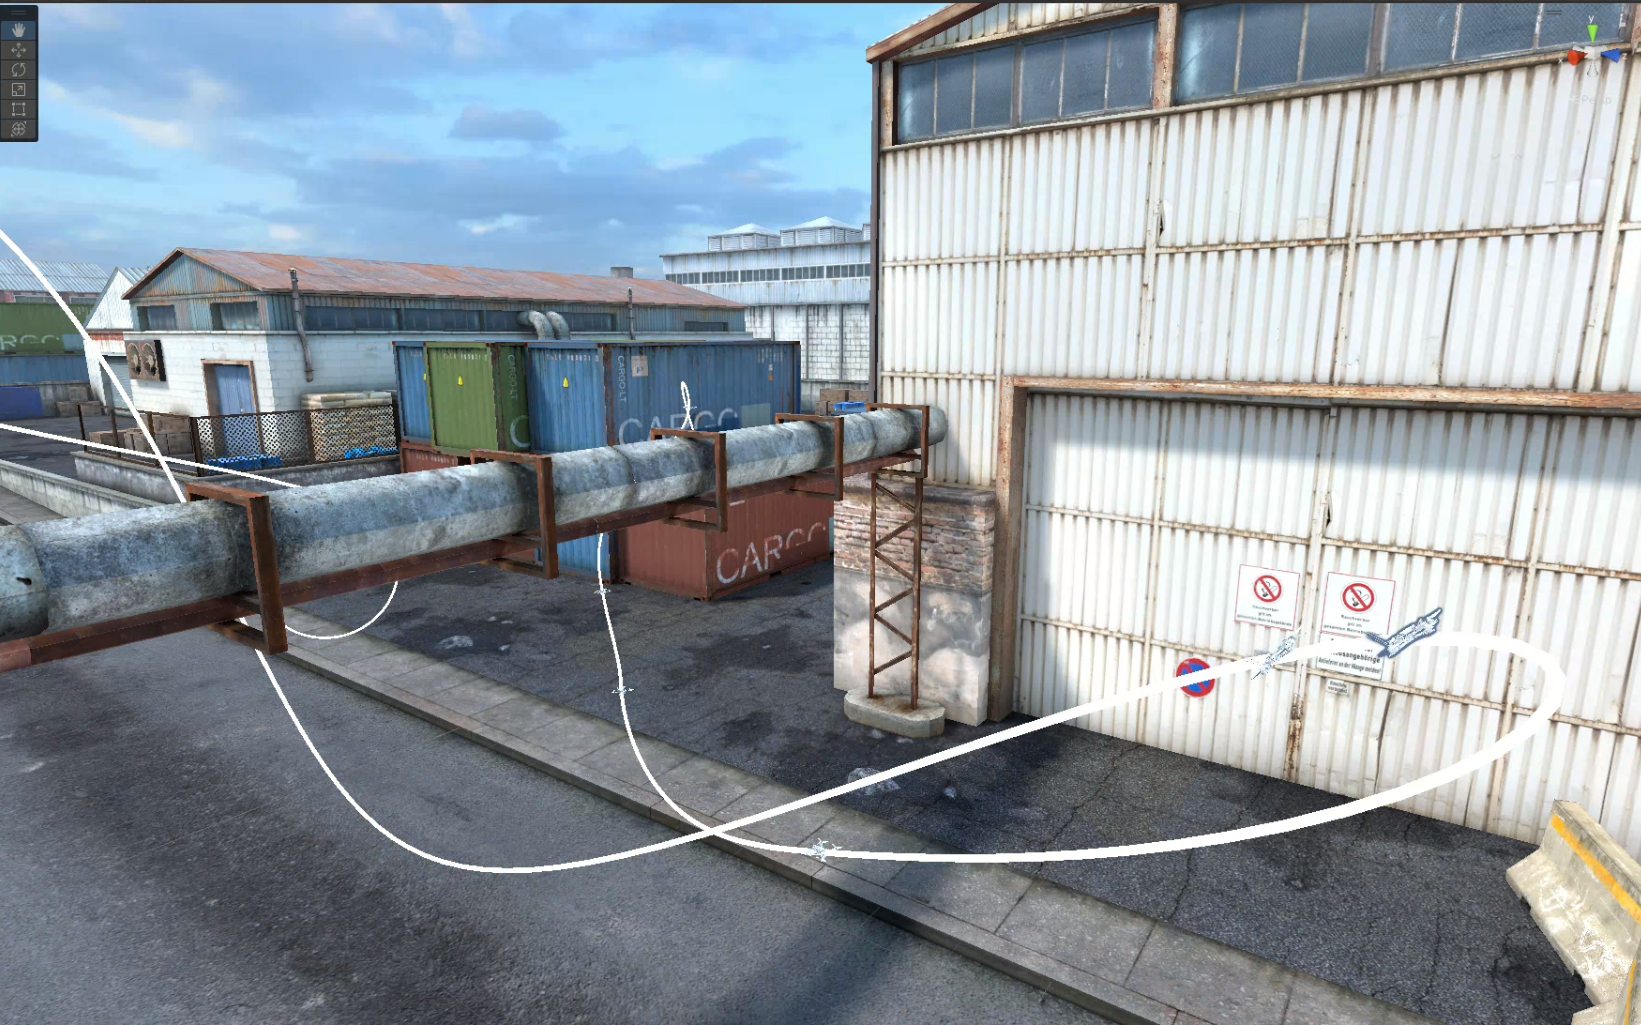
\includegraphics[width=0.75\linewidth]{data/rotation.png}
  \caption{There are two quadrotors shown in the foreground of this frame. The left quadrotor is a constraint with rotation enforced. The right quadrotor with a faint blue outline is tracking the trajectory, and has just passed the constraint. It is pitched back substantially, which reflects the pitch angle of the constraint as expected. This is part of the same trajectory shown in Figure \ref{fig:overview}.}
  \label{fig:rotation}
\end{figure}

Two of the constraints shown in Figure \ref{fig:overview} fix the quadrotor's rotation, and the left leave it unconstrained. The first of these is the second constraint, featured in Figure \ref{fig:constraint}, which requires that the quadrotor has a pitch of \qty{0}{deg} and a roll of \qty{20}{deg} to the right. Figure \ref{fig:onboard} is a frame taken from a video of a quadrotor tracking the trajectory, from the perspective of a camera onboard the quadrotor \footnote{See video: https://drive.google.com/file/d/1Q52Q4-DGpkiKXSAfPmdqt95fDZHyswE8/view?usp=sharing}. The frame is taken when the quadrotor is in the vicinity of this second constraint, and it is apparent that the trajectory respects the roll angle constraint here. The second constraint that enforces the quadrotor's rotation is after the quadrotor passes under the elevated pipe, and is pictured in Figure \ref{fig:rotation}. Although it is difficult to discern because of the background, there are two quadrotor models shown in the foreground of this figure. The one to the left is the constraint in question, and the one to the right with a faint blue outline is the quadrotor just after passing through this constraint. The constraint requires the quadrotor to pitch back significantly, and the figure confirms that the quadrotor does assume the correct rotation at the constraint \footnote{See video: https://drive.google.com/file/d/1RPgdxUxGlWry4A1bbcxrVOgbvc1ThxMU/view?usp=sharing}.

\begin{figure}
  \begin{minipage}{0.5\linewidth}
    \includegraphics[width=\linewidth]{data/3angles_25speeds.png}
    \includegraphics[width=\linewidth]{data/5angles_25speeds.png}
    \includegraphics[width=\linewidth]{data/25angles_25speeds.png}
  \end{minipage}
  \begin{minipage}{0.5\linewidth}
    \includegraphics[width=\linewidth]{data/1speed_25angles.png}
    \includegraphics[width=\linewidth]{data/10speeds_25angles.png}
    \includegraphics[width=\linewidth]{data/100speeds_25angles.png}
  \end{minipage}
  \caption{Six different trajectories generated from the same four constraints (in red) with unconstrained rotation, using Algorithm \ref{alg:greedy}. They are generated using different direction sets $A$ and speed sets $S$. $A$ and $S$ contain linearly spaced values in the intervals $[0, 2\pi)$ and $[0, v_{\max} = 25]$, respectively. In the first column, from top to bottom, $(|A|, |S|)$ is $(3, 25)$, $(5, 25)$, and $(25, 25)$. In the second column, from top to bottom, $(|A|, |S|)$ is $(25, 1)$, $(25, 10)$, and $(25, 100)$.}
  \label{fig:greedy}
\end{figure}

Figure \ref{fig:greedy} shows results for generating a simple, four constraint trajectory with unconstrained rotation using Algorithm \ref{alg:greedy} with varying parameters. Note that these are the same constraints as in Figure \ref{fig:naive}, which shows a trajectory generated using Algorithm \ref{alg:naive}. The two figures suggest that Algorithm \ref{alg:greedy} performs much better, as the trajectories it generates take an intuitive route through the constraints, whereas the trajectory generated by Algorithm \ref{alg:naive} appears to have excessively long tails after each segment for the quadrotor to decelerate. In Figure \ref{fig:greedy}, the left column shows results for generating with a fixed speed set $S$ and an increasingly large direction set $A$ (from top to bottom), and the right column shows results for generating with a fixed direction set $A$ and an increasingly large speed set $S$ (from top to bottom). As expected, the trajectories generated with larger $A$ and $S$ appear smoother. While the effect of $S$ is clear, the effect of $A$ is demonstrated well by the top left image, where the trajectory visibly compensates for the lack of velocity vectors to choose from. The algorithm appears to be more sensitive to $S$ than $A$, but it should be noted that the choice of $v_{\max}$ could significantly impact this, which is $v_{\max} = 25$ in these tests. $v_{\max}$ influences the granularity of speeds in $S$, since the implementation chooses linearly spaced values in $[0, v_{\max}]$.

\begin{table}
  \centering
  \begin{tabular}{|l|l|l|l|} \hline
    $|\textbf{A}|$ & $|\textbf{S}|$ & \textbf{Total cost} & \textbf{Generation time [s]} \\ \hline
    3 & 25 & 5051 & 0.71 \\ \hline
    5 & 25 & 5365 & 1.17 \\ \hline
    25 & 25 & 5866 & 5.54 \\ \hline
    25 & 1 & 7289 & 0.32 \\ \hline
    25 & 10 & 6506 & 2.24 \\ \hline
    25 & 100 & 5663 & 22.23 \\ \hline
  \end{tabular}
  \caption{This table gives the total trajectory cost, rounded to an integer, and generation time for each of the trajectories shown in Figure \ref{fig:greedy}. $|A|$ and $|S|$ are the sizes of the direction set and speed set, respectively.}
  \label{table:total}
\end{table}

\begin{table}
  \centering
  \begin{tabular}{|l|l|l|l|l|} \hline
    \textbf{Segment} & \textbf{Feasible [\%]} & \textbf{Mean cost} & \textbf{Min cost} & \textbf{Max cost} \\ \hline
    1 & 91 & 135 & 2 & 753 \\ \hline
    2 & 99 & 22 & 5 & 71 \\ \hline
    3 & 79 & 153 & 10 & 820 \\ \hline
    4 & 52 & 112 & 16 & 421 \\ \hline
    5 & 29 & 26 & 2 & 127 \\ \hline
    6 & 26 & 1093 & 14 & 3424 \\ \hline
    7 & 43 & 158 & 21 & 452 \\ \hline
    8 & 100 & 46 & 46 & 46 \\ \hline
  \end{tabular}
  \caption{This table gives statistics related to the generation of the trajectory shown in Figure \ref{fig:overview}. For each trajectory segment, the percentage of motion primitive candidates which are feasible is given, along with the mean, minimum, and maximum cost among the feasible candidates, rounded to an integer. These cost values are the cost of the current segment; they do not include the cost of the induced trajectory. The total generation time for this trajectory was 57.67 s.}
  \label{table:segments}
\end{table}

Table \ref{table:total} gives information about the generation of the trajectories shown in Figure \ref{fig:greedy}. The generation time increases roughly linearly with $|A|$ and $|S|$, which is as expected. The total trajectory cost decreases as $|S|$ is increased, which is also expected, but interestingly the cost increases as $|A|$ increases. Since the trajectories do appear smoother as $|A|$ increases, this suggests that jerk may not be the ideal cost function for freestyle trajectories, and alternatives like acceleration could be explored in future work. This could also indicate that keeping the cost of the trajectory low over a short time horizon is more important than minimizing the cost globally in making the trajectory appear natural and smooth to a human. Table \ref{table:segments} gives information about the generation of the trajectory shown in Figure \ref{fig:overview}. The proportion of feasible motion primitives varies considerably at each segment index. The distributions of motion primitive costs also have significant variation. The costs are generally much lower than those in Table 1, which is likely related to differences in the distances and durations between constraints in the two trajectories.

\section{Conclusion}

This project develops a graphical interface and algorithm for freestyle trajectory generation, which is a novel contribution in that freestyle trajectories have not been explicitly considered in the literature before. The trajectory generation algorithm is designed with freestyle trajectories in mind, which is achieved by allowing users to set expressive constraints with a fixed rotation, and by ensuring that trajectories are smooth. It applies the work of Mueller et al. on motion primitives to produce complex trajectories, demonstrating that motion primitives are an effective building block, and that reasonable results for this problem can be achieved by combining them with a simple heuristic and exhaustive search, without needing to resort to more complicated trajectory generation methods as described in the literature. The graphical tool allows users to create these trajectories using a natural interface, without needing much or any knowledge of how the generation process works. It expands upon the work of Mceowen et al. by not restricting trajectories to 2D, and unlocking the full capabilities of quadrotors in doing so. Being able to design and inspect trajectories in a realistic 3D environment is an important step toward autonomous freestyle flight, and the results suggest that this approach is a promising way of doing so.

There are many potential directions for future work on this project. First, as mentioned previously, is adding yaw rotation to the trajectories. Yaw constraints could be implemented in several different ways, including by enforcing the yaw rotation at rotation constraints $R_i$, or by setting it to keep the camera pointed in the direction of travel. Other future work related to trajectory generation includes extending the proposed algorithm to optimize over trajectory segment durations instead of having the user set these, exploring alternative objective functions such as minimizing acceleration, which may better represent the human notion of a smooth trajectory, and using another approach entirely like a global optimization algorithm. Applying machine learning to automatically generate constraints that lead to \quotes{interesting} trajectories could even be explored. Beyond the trajectory generation algorithm, there are a myriad of improvements that could be made to the graphical interface, including removing the dependency on the Unity editor, making it more user friendly, and displaying more feedback to the user. Finally, the feasibility of the trajectories could be verified by tracking them in simulation or with a real quadrotor using existing control algorithms.

Drones are more prevalent and capable than ever before, and autonomy has played a large role in this. This project represents a small contribution toward making autonomy more accessible, through graphical tools, and does so for the context of freestyle flight, which is a great example of how drones can both be fun and add value at the same time. Bringing autonomy to this domain has the potential to create new opportunities for drone users, while simultaneously providing a great way to test and expand the limits of what autonomous drones can do.

\section{Acknowledgements}

I'd like to thank Professor Kincaid for his help in guiding the direction of this project and for providing helpful feedback throughout the semester. I'd also like to thank my classmates for an enjoyable semester. Finally, I'd like to thank my first year writing seminar professor, Dr. Penman, for giving me the skills, and more importantly the confidence, to write a paper of this magnitude.


\bstctlcite{bstctl:etal, bstctl:nodash, bstctl:simpurl}
\bibliographystyle{IEEEtranS}
\bibliography{references}

\end{document}
